\section{Introduction}
\label{sec:intro}

\begin{figure}[t]
    \centering
    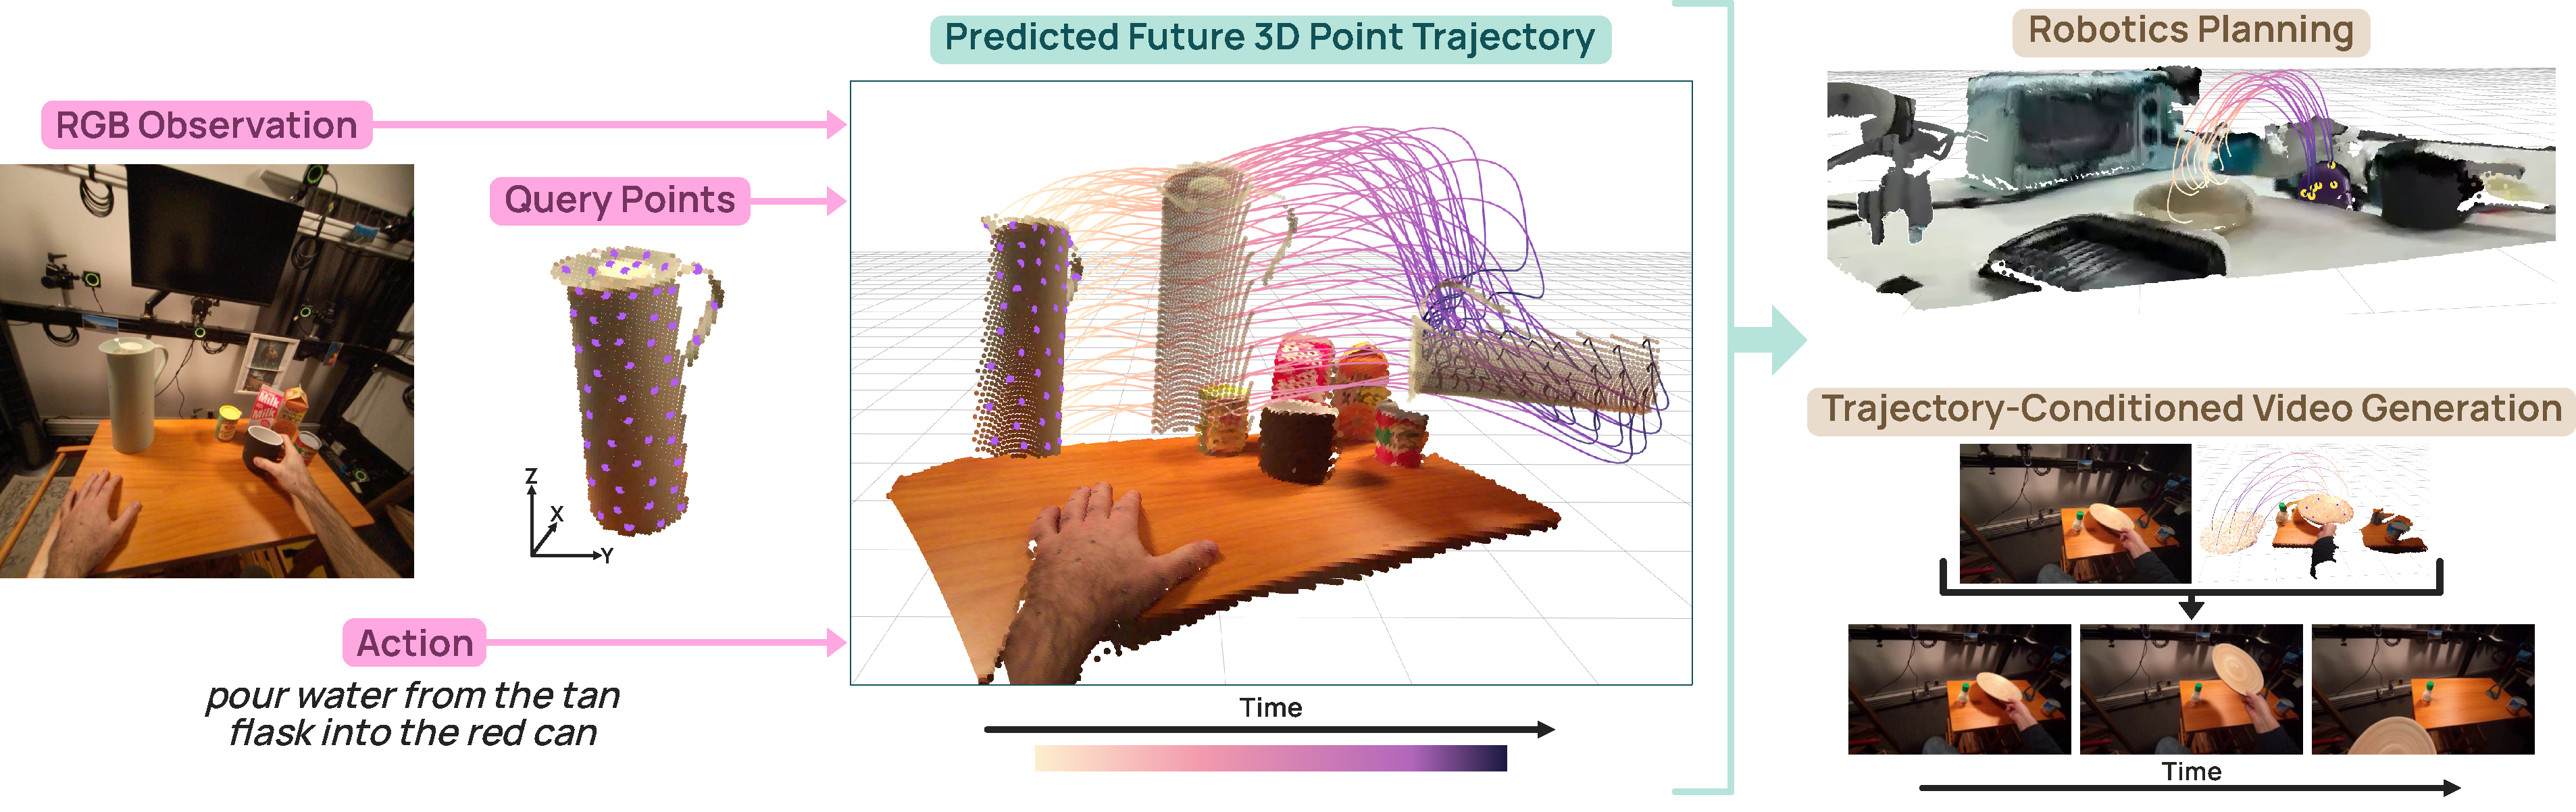
\includegraphics[width=\linewidth]{figures/Teaser_3.pdf}
    \caption{
        \textbf{Overview.} We introduce the task of goal-conditioned 3D point motion prediction. 
        Given initial 3D query points on an object, history RGB observations, and a language description of the future action, our model predicts the future 3D positions of all queried points in a metric world coordinate frame. 
        We show that pretraining this motion prediction task produces a transferable motion representation for downstream applications, including robotics planning and  video generation. }
    \label{fig:teaser}
\end{figure}

Psychologists like James J. Gibson have long argued that motion is core to perception, hypothesizing that motion informs an observer how they and other objects move through space, explains object occlusion and permanence, and identifies affordances~\cite{gibson2014ecological}. In the 70s, Ullman formalized motion perception as a computational problem~\cite{ullman1979interpretation}, with Lucas and Kanade providing an algorithm for estimating motion to enable tracking as optical flow~\cite{lucas1981iterative}. Although such methods have improved~\cite{raft, doersch2022tapvid, cotracker3}, they remain primarily focused on estimating motion that has \textit{already} occurred. Many real-world applications instead require \emph{forecasting} how motion will unfold. In robotics, an agent must anticipate how its actions will move objects through the scene~\cite{finn2017deepvisualforesight, track2act}. In video generation, realistic synthesis requires precise forecasting of the future motion of objects~\cite{nvidia2025cosmos, bruce2024genie}. 


Building a general motion forecasting model imposes several requirements on the representation used for motion. First, the representation should be \textit{class-agnostic}: it should not depend on templates tailored to humans, hands, rigid objects, or any other fixed categories. Second, it should be \textit{view-stable}: the same underlying motion should be represented consistently across different cameras, from static surveillance footage to egocentric robot videos and moving outdoor platforms. Third, it should expose \textit{physical structure} in a form that downstream systems can use directly. 
Existing approaches of motion prediction only partially satisfy these requirements. While \textit{pixels} provide a rich rendering of possible futures~\cite{wan22, nvidia2025cosmos, bruce2024genie}, they are expensive to generate and often difficult to utilize directly in downstream applications.
Many applications instead require explicit geometric and physical quantities, such as object pose~\cite{traj2action, wen2023bundlesdf, vidbot} or particle-level dynamics~\cite{li2018particledynamics, sanchez2020graphnetworksimulators}.
\textit{Parametric 3D models} (for humans~\cite{chen2023humanmac}, hands~\cite{bi2025hrdthumanmanipulationenhanced}, or rigid objects~\cite{soraki2026objectforesightpredictingfuture3d}) are useful for such applications but remain restricted to specific categories and embodiments. 
\textit{2D point trajectories} are more category-agnostic, but image-plane coordinates entangle object motion with camera ego-motion and viewpoint change, making them difficult to disentangle from videos and transfer across domains~\cite{track2act, thakkar2026forecastingmotion}. 

We argue that \textit{object-attached 3D points in world coordinates} provide a suitable representation for general motion forecasting. A sparse set of surface points moving through 3D space can describe the motion of rigid, articulated, or deformable objects without assuming a category-specific template. Because 3D points share a world frame, the same physical motion can remain stable across cameras, viewpoints, and capture settings. Additionally, many task-relevant quantities can be expressed as the motion of 3D points, from the pose change of a robot gripper~\cite{vidbot} to particle trajectories in physical simulation~\cite{li2018particledynamics, sanchez2020graphnetworksimulators}. 
Finally, by focusing only on object-attached points, the prediction target remains compact while still capturing the motion relevant for physical interaction.

We formalize this idea as the task of \textit{goal-conditioned 3D point motion prediction} (Fig.~\ref{fig:teaser}). Given a short history of visual observations, a set of initial 3D query points on an object of interest, and a language description of the intended goal, the model predicts the future 3D trajectory of each query point over time. The language instruction disambiguates among plausible futures and reduces the search space of possible future states.


We present the full stack needed to study this task at scale: \textbf{a scalable data curation pipeline}, \textbf{a novel prediction model}, and \textbf{a human-verified benchmark}. The first challenge is 3D motion supervision data. Existing video datasets with 3D capture are small and domain-limited~\cite{hot3d, koppula2024tapvid3d, liu2022hoi4d}, while internet videos provide scale and diversity but lack 3D annotations. We therefore develop an automatic annotation pipeline for robustly extracting object-grounded 3D point trajectories from unconstrained videos. Applying this pipeline to roughly 1.16M video clips yields MolmoMotion-1M, the largest corpus of action-described, object-grounded 3D point trajectories. We additionally introduce \benchmarkname{}, a benchmark for 3D motion forecasting spanning 111 object categories and 61 motion types. The benchmark uses ground-truth 3D capture where available and human-verified 3D tracks otherwise, providing a reliable testbed for evaluating motion prediction.

We introduce \modelname, a general motion prediction model pretrained on the MolmoMotion-1M dataset. We train two complementary classes of motion prediction models. The first predicts future trajectories autoregressively as coordinate sequences; the second predicts future motion with flow matching as a continuous trajectory distribution. 
Experiments show \modelname accurately forecast diverse motion types and generalize across a wide range of scenes and instructions, and significantly outperforms all existing motion prediction methods in \benchmarkname{}.


Finally, we validate 3D point forecasting as a useful task: \modelname transfers effectively to downstream applications.
Because object trajectories in 3D world space are largely embodiment-agnostic~\cite{track2act, dharmarajan2025dream2flow}, the motion prior learned from internet-scale human video can transfer naturally to robotics planning. We show that this prior improves sample efficiency, closed-loop success, and generalization to unseen objects and scenes in the MolmoSpaces pick-and-place task~\cite{molmospaces}, and adapts efficiently to real-world robot videos from DROID~\cite{droid}.
\modelname can also guide video generation. When its predicted trajectories are used to condition a lightweight 3D-track-conditioned image-to-video model~\cite{gu2025diffusionasshader}, the generated videos exhibit more realistic motion than those produced directly by much larger image-to-video models~\cite{wan22}, while also improving multiple quantitative video-quality metrics.
